\documentclass{article}

\usepackage{euler}

\usepackage[
  paperwidth=9in,
  paperheight=4.5in,
  layoutwidth=9in,
  layoutheight=4.5in,
  width=9in,
  height=4.5in,
  margin=0in,
]{geometry}

\usepackage{tikz}
\usetikzlibrary{intersections}
\usetikzlibrary{shapes.geometric}

\begin{document}
\thispagestyle{empty}
\noindent
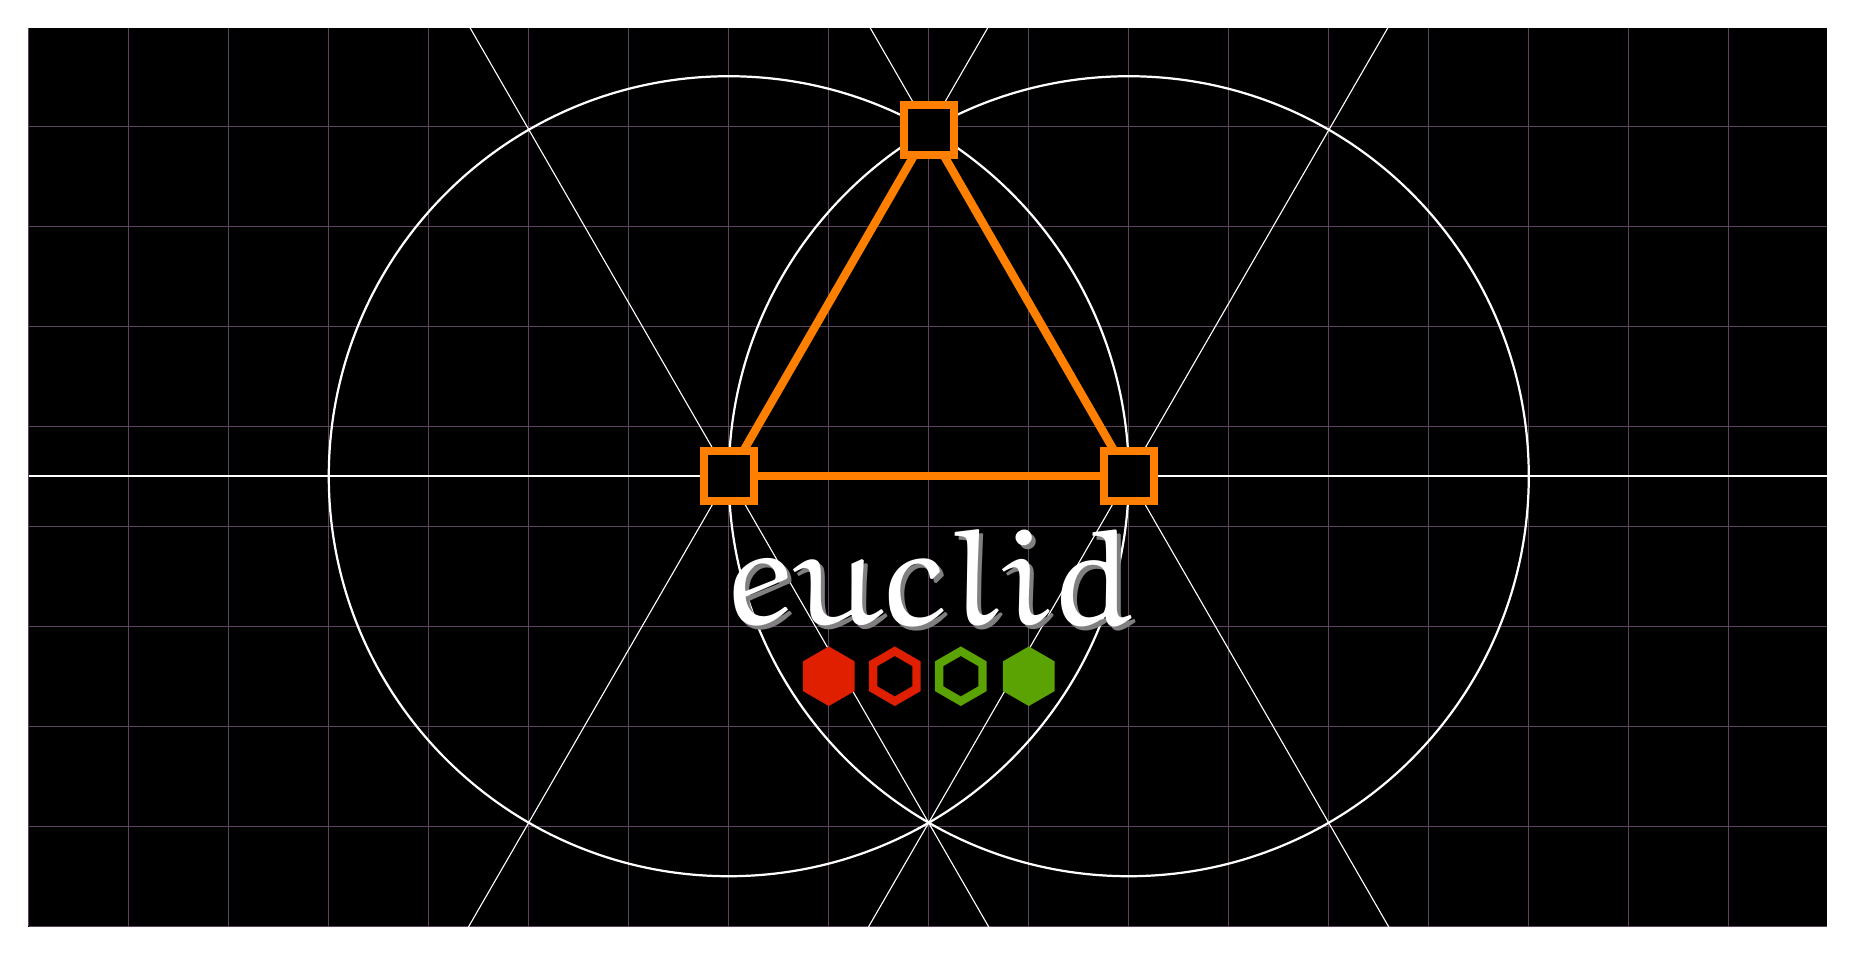
\begin{tikzpicture}
  \draw[fill=black] (0, 0) rectangle (8.99in, 4.49in);
  \draw[
    thin,
    color={rgb:red,136;green,101;blue,141},
    step=0.5in,
  ] (0, 0) grid (8.99in, 4.49in);

  \draw[name path=H,thick,white] (0.00in, 2.25in) -- (9in, 2.25in);
  \draw[name path=L,thick,white] (3.5in, 2.25in) circle [radius=2in];
  \draw[name path=R,thick,white] (5.5in, 2.25in) circle [radius=2in];

  \path[name intersections={of=H and R}];
  \coordinate (l) at (intersection-1);

  \path[name intersections={of=H and L}];
  \coordinate (r) at (intersection-2);

  \path[name intersections={of=L and R}];
  \coordinate (u) at (intersection-1);
  \coordinate (d) at (intersection-2);

  \draw[thin,white,shorten >=-4.5in,shorten <=-4.5in] (l) -- (u);
  \draw[thin,white,shorten >=-4.5in,shorten <=-4.5in] (r) -- (u);
  \draw[thin,white,shorten >=-4.5in,shorten <=-4.5in] (l) -- (d);
  \draw[thin,white,shorten >=-4.5in,shorten <=-4.5in] (r) -- (d);

  \draw[orange,line width=3pt] (l) -- (r);
  \draw[orange,line width=3pt] (l) -- (u);
  \draw[orange,line width=3pt] (r) -- (u);

  \node[
    rectangle,
    fill=black,
    draw=orange,
    inner sep=0pt,
    line width=3pt,
    minimum width=0.25in,
    minimum height=0.25in,
  ] at (l) {};

  \node[
    rectangle,
    fill=black,
    draw=orange,
    inner sep=0pt,
    line width=3pt,
    minimum width=0.25in,
    minimum height=0.25in,
  ] at (r) {};

  \node[
    rectangle,
    fill=black,
    draw=orange,
    inner sep=0pt,
    line width=3pt,
    minimum width=0.25in,
    minimum height=0.25in,
  ] at (u) {};

  % Drop shadow
  \node[black!50!white] at (4.52in,1.73in) {
    \fontsize{50}{50}\selectfont $euclid$
  };
  \node[color=white] at (4.5in,1.75in) {
    \fontsize{50}{50}\selectfont $euclid$
  };

  \node[
    draw={rgb:red,215;green,30;blue,0},
    fill={rgb:red,215;green,30;blue,0},
    line width=3pt,
    regular polygon,
    regular polygon sides=6,
    minimum size=0.25in,
    rotate=90,
  ] at (4.0in,1.25in) {};

  \node[
    draw={rgb:red,215;green,30;blue,0},
    fill=black,
    line width=3pt,
    regular polygon,
    regular polygon sides=6,
    minimum size=0.25in,
    rotate=90,
  ] at (4.33in,1.25in) {};

  \node[
    draw={rgb:red,93;green,168;blue,2},
    fill=black,
    line width=3pt,
    regular polygon,
    regular polygon sides=6,
    minimum size=0.25in,
    rotate=90,
  ] at (4.66in,1.25in) {};

  \node[
    draw={rgb:red,93;green,168;blue,2},
    fill={rgb:red,93;green,168;blue,2},
    line width=3pt,
    regular polygon,
    regular polygon sides=6,
    minimum size=0.25in,
    rotate=90,
  ] at (5.0in,1.25in) {};
\end{tikzpicture}
\end{document}
